\usetikzlibrary{matrix, positioning}

\definecolor{c1}{HTML}{9ACFC6}
\definecolor{c2}{HTML}{DABBD6}
\definecolor{c3}{HTML}{CBDCB9}
\definecolor{c4}{HTML}{9AC3E1}
\definecolor{c5}{HTML}{DEBBA5}
\definecolor{c6}{HTML}{C4DDE5}

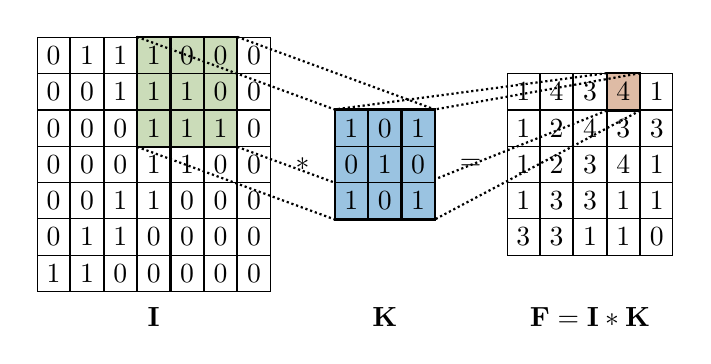
\begin{tikzpicture}
	\matrix (mtr) [matrix of nodes,row sep=-\pgflinewidth, nodes={draw}]
	{
		0 & 1 & 1 & |[fill=c3]| 1 & |[fill=c3]| 0 & |[fill=c3]| 0 & 0\\
		0 & 0 & 1 & |[fill=c3]| 1 & |[fill=c3]| 1 & |[fill=c3]| 0 & 0\\
		0 & 0 & 0 & |[fill=c3]| 1 & |[fill=c3]| 1 & |[fill=c3]| 1 & 0\\
		0 & 0 & 0 & 1 & 1 & 0 & 0\\
		0 & 0 & 1 & 1 & 0 & 0 & 0\\
		0 & 1 & 1 & 0 & 0 & 0 & 0\\
		1 & 1 & 0 & 0 & 0 & 0 & 0\\
	};

	\draw[thick, black] (mtr-1-4.north west) rectangle (mtr-3-6.south east);

	\node [below= of mtr-5-4.south] (lm) {$\bf I$};

	\node[right = 0.2em of mtr] (str) {$*$};

	\matrix (K) [right=0.2em of str,matrix of nodes,row sep=-\pgflinewidth, nodes={draw, fill=c1}]
	{
		1 & 0 & 1 \\
		0 & 1 & 0 \\
		1 & 0 & 1 \\
	};
	\node [below = of K-3-2.south] (lk) {$\bf K$};

	\node [right = 0.2em of K] (eq) {$=$};

	\matrix (ret) [right=0.2em of eq,matrix of nodes,row sep=-\pgflinewidth, nodes={draw}]
	{
		1 & 4 & 3 & |[fill=c5]| 4 & 1\\
		1 & 2 & 4 & 3 & 3\\
		1 & 2 & 3 & 4 & 1\\
		1 & 3 & 3 & 1 & 1\\
		3 & 3 & 1 & 1 & 0\\
	};
	\node [below = of ret-4-3.south] (lim) {${\bf F} = {\bf I} * {\bf K}$};

	\draw[thick, black] (ret-1-4.north west) rectangle (ret-1-4.south east);

	\draw[densely dotted, black, thick] (mtr-1-4.north west) -- (K-1-1.north west);
	\draw[densely dotted, black, thick] (mtr-3-4.south west) -- (K-3-1.south west);
	\draw[densely dotted, black, thick] (mtr-1-6.north east) -- (K-1-3.north east);
	\draw[densely dotted, black, thick] (mtr-3-6.south east) -- (K-3-3.south east);

	\draw[densely dotted, black, thick] (ret-1-4.north west) -- (K-1-1.north west);
	\draw[densely dotted, black, thick] (ret-1-4.south west) -- (K-3-1.south west);
	\draw[densely dotted, black, thick] (ret-1-4.north east) -- (K-1-3.north east);
	\draw[densely dotted, black, thick] (ret-1-4.south east) -- (K-3-3.south east);

	\matrix (K) [right=0.2em of str,matrix of nodes,row sep=-\pgflinewidth, nodes={draw, fill=c4}]
	{
		1 & 0 & 1 \\
		0 & 1 & 0 \\
		1 & 0 & 1 \\
	};

	\draw[thick, black] (K-1-1.north west) rectangle (K-3-3.south east);

	% \node[anchor=south east, inner sep=0.01em, blue] at (mtr-1-4.south east) (xx) {\scalebox{.5}{$\times 1$}};
	% \node[anchor=south east, inner sep=0.01em, blue] at (mtr-1-5.south east) (xx) {\scalebox{.5}{$\times 0$}};
	% \node[anchor=south east, inner sep=0.01em, blue] at (mtr-1-6.south east) (xx) {\scalebox{.5}{$\times 1$}};
	% \node[anchor=south east, inner sep=0.01em, blue] at (mtr-2-4.south east) (xx) {\scalebox{.5}{$\times 0$}};
	% \node[anchor=south east, inner sep=0.01em, blue] at (mtr-2-5.south east) (xx) {\scalebox{.5}{$\times 1$}};
	% \node[anchor=south east, inner sep=0.01em, blue] at (mtr-2-6.south east) (xx) {\scalebox{.5}{$\times 0$}};
	% \node[anchor=south east, inner sep=0.01em, blue] at (mtr-3-4.south east) (xx) {\scalebox{.5}{$\times 1$}};
	% \node[anchor=south east, inner sep=0.01em, blue] at (mtr-3-5.south east) (xx) {\scalebox{.5}{$\times 0$}};
	% \node[anchor=south east, inner sep=0.01em, blue] at (mtr-3-6.south east) (xx) {\scalebox{.5}{$\times 1$}};

\end{tikzpicture}